\documentclass[12pt,german]{article}

\usepackage[left=2cm, right=2cm, top=2cm, bottom=3.5cm, landscape=false]{geometry}

\usepackage{graphicx}
\usepackage{float}

\usepackage{tabularx}
\newcolumntype{R}{>{\raggedleft\arraybackslash}X}
\newcolumntype{L}{>{\raggedright\arraybackslash}X}
\newcolumntype{C}{>{\centering\arraybackslash}X}
\usepackage{booktabs}
\usepackage{dcolumn}
\usepackage{multirow}

\usepackage[ngerman]{babel}

\usepackage{amsmath}

\title{\vspace{-1.5cm}Protokoll Kritisches Experiment}
\author{Fuchs, Gutmann, Kosbab, Kowal, Steindorf, Fälker, Richter}
\setlength\parindent{0pt}


\begin{document}
    \maketitle
    \tableofcontents

    \section{Kurzbeschreibung des Versuches}
    \begin{itemize}
        \item Zu Beginn wird die Funktionsfähigkeit der Sicherheitssysteme getestet, indem manuell eine Totalabschaltung ausgelöst wird.
        \item Die Anfahrneutronenquelle wird eingefahren und das Signal \glqq Kernhälften zusammen\grqq  mit dem Schalter \glqq  Simulation Kernhälften zusammen\grqq überbrückt, um auch bei getrennten Kernhälften eine Veränderung der Steuerstäbe zu ermöglichen.
        \item Es wird die Untergrundaktivität bei ein- und ausgefahrenen Steuerstäben gemessen.
        \item Anschließend wird die untere Kernhälfte zunächst um 100 Digits angehoben, wonach die Impulsrate mit ein- und ausgefahrenen Steuerstäben gemessen wird.
        \item Aus den Impulsraten wird berechnet, um wie viele Digits die Kernhälfte erneut angehoben werden darf.
        \item Die letzten beiden Schritte werden wiederholt, bis durch Extrapolation der Schnittpunkte mit der X-Achse die Ungleichung \(X_\text{krit, aus}(i) < X_\text{max} < X_\text{krit, ein}(i)\) zuverlässig erfüllt ist.
    \end{itemize}

    \newpage

    \section{Messwerttabellen}

    Zu Beginn werden die Impulsraten für beide Weitbereichsmesskanäle gemessen, wobei die untere Kernhälfte komplett abgesenkt ist.

    \begin{table}[H]
        \centering
        \begin{tabularx}{\textwidth}{L|L|R|R|R|R}
            \toprule
            & \textbf{Steuerstabs\newline stellung} & \textbf{Messung 1} & \textbf{Messung 2} & \textbf{Messung 3} & \textbf{Mittelwert \(N_0\)} \\
            \midrule
            \multirow{2}{*}{WB 1} & ein (0) & 7.4 & 7.3 & 7.6 & 7.43 \\
            & aus (4000) & 9.4 & 9.3 & 9.6 & 9.43 \\
            \midrule
            \multirow{2}{*}{WB 2} & ein (0) & 6.9 & 6,6 & 6,7 & 6,73 \\
            & aus (4000) & 10,4 & 10,3 & 10,1 & 10,26 \\
            \bottomrule
        \end{tabularx}
        \caption{Bestimmung der Ausgangswerte \(N_0\)}
    \end{table}

    Die originalen Messwerttabellen sind im Anhang aufgeführt, da jedoch ein Fehler in der Berechnung des Multiplikationsfaktors bei Weitbereichsmesskanal 1 enthalten ist, sind die Tabellen an dieser Stelle korrigiert gegeben.

    \begin{table}[H]
        \begin{tabularx}{\textwidth}{L|C|R|R|R|R|R|R|R}
            \toprule
            Hubhöhe & \centering Stab- & \multicolumn{3}{c|}{Zählraten} &  &  &  &  \\
            $[x_i / dgts.]$ & \centering stellung & \centering $N_{i, 1}$ & \centering $N_{i, 2}$ & \centering $\overline{N_i}$ & \centering $N_0 / \overline{N_i}$ & \centering $k_i$ & \centering $M_i$ & \multicolumn{1}{c}{$\rho_i$} \\
            \midrule
            \multirow{2}{*}{  0} & ein & \multicolumn{3}{r|}{ 7.43} & 1.000 & 0.945 &  18.18 & -0.0582 \\
                                 & aus & \multicolumn{3}{r|}{ 9.43} & 1.000 & 0.945 &  18.18 & -0.0582 \\
            \midrule
            \multirow{2}{*}{100} & ein &    8.5 &    8.6 &     8.55 & 0.869 & 0.952 &  20.92 & -0.0502 \\
                                 & aus &   10.8 &   10.7 &    10.75 & 0.878 & 0.952 &  20.70 & -0.0508 \\
            \midrule
            \multirow{2}{*}{200} & ein &    9.8 &    9.9 &     9.85 & 0.755 & 0.959 &  24.10 & -0.0433 \\
                                 & aus &   13.7 &   13.9 &    13.80 & 0.684 & 0.962 &  26.60 & -0.0391 \\
            \midrule
            \multirow{2}{*}{300} & ein &   12.5 &   12.7 &    12.60 & 0.590 & 0.968 &  30.86 & -0.0335 \\
                                 & aus &   18.5 &   18.3 &    18.40 & 0.513 & 0.972 &  35.46 & -0.0290 \\
            \midrule
            \multirow{2}{*}{400} & ein &   19.2 &   18.8 &    19.00 & 0.391 & 0.979 &  46.51 & -0.0220 \\
                                 & aus &   36.8 &   36.4 &    36.60 & 0.258 & 0.986 &  70.42 & -0.0144 \\
            \midrule
            \multirow{2}{*}{450} & ein &   31.1 &   30.1 &    30.60 & 0.243 & 0.987 &  75.19 & -0.0135 \\
                                 & aus &   87.4 &   88.6 &    88.00 & 0.107 & 0.994 & 169.49 & -0.0059 \\
            \midrule
                             500 & ein &   52.3 &   52.0 &    52.15 & 0.143 & 0.992 & 128.21 & -0.0079 \\
            \bottomrule
        \end{tabularx}
        \caption{Messwerte für Weitbereichsmesskanal 1}
    \end{table}

    \begin{table}[H]
        \begin{tabularx}{\textwidth}{L|C|R|R|R|R|R|R|R}
            \toprule
            Hubhöhe & \centering Stab- & \multicolumn{3}{c|}{Zählraten} &  &  &  &  \\
            $[x_i / dgts.]$ & \centering stellung & \centering $N_{i, 1}$ & \centering $N_{i, 2}$ & \centering $\overline{N_i}$ & \centering $N_0 / \overline{N_i}$ & \centering $k_i$ & \centering $M_i$ & \multicolumn{1}{c}{$\rho_i$} \\
            \midrule
            \multirow{2}{*}{  0} & ein & \multicolumn{3}{r|}{ 6.73} & 1.000 & 0.945 &  18.18 & -0.0582 \\
                                 & aus & \multicolumn{3}{r|}{10.27} & 1.000 & 0.945 &  18.18 & -0.0582 \\
            \midrule
            \multirow{2}{*}{100} & ein &    8.2 &    7.8 &     8.00 & 0.842 & 0.954 &  21.60 & -0.0486 \\
                                 & aus &   11.9 &   11.5 &    11.70 & 0.877 & 0.952 &  20.70 & -0.0508 \\
            \midrule
            \multirow{2}{*}{200} & ein &    9.1 &    9.2 &     9.15 & 0.736 & 0.960 &  24.69 & -0.0422 \\
                                 & aus &   14.8 &   15.2 &    15.00 & 0.684 & 0.962 &  26.53 & -0.0392 \\
            \midrule
            \multirow{2}{*}{300} & ein &   11.9 &   11.6 &    11.75 & 0.573 & 0.969 &  31.75 & -0.0325 \\
                                 & aus &   21.5 &   20.8 &    21.15 & 0.485 & 0.973 &  37.45 & -0.0274 \\
            \midrule
            \multirow{2}{*}{400} & ein &   17.8 &   18.4 &    18.10 & 0.372 & 0.980 &  49.02 & -0.0208 \\
                                 & aus &   40.8 &   41.3 &    41.05 & 0.250 & 0.986 &  72.46 & -0.0140 \\
            \midrule
            \multirow{2}{*}{450} & ein &   28.5 &   29.1 &    28.80 & 0.234 & 0.987 &  78.12 & -0.0130 \\
                                 & aus &   96.7 &   99.3 &    98.00 & 0.105 & 0.994 & 172.41 & -0.0058 \\
            \midrule
                             500 & ein &   49.6 &   49.2 &    49.40 & 0.136 & 0.993 & 133.33 & -0.0076 \\
            \bottomrule
        \end{tabularx}
        \caption{Messwerte für Weitbereichsmesskanal 2}
    \end{table}

    \section{Berechnung der Anhebung}
    Dadurch, dass die Neutronendichte in einem kritischen Reaktor bei eingefahrener Anfahrneutronenquelle gegen Unendlich strebt, geht gleichermaßen der reziproke Wert der Neutronendichte gegen Null.
    Da die Impulsrate eines Neutronenmesskanals direkt proportional zur Neutronendichte ist, kann diese als Messgröße verwendet werden.
    Ebenfalls kann die Größe normiert werden, indem statt dem reziproken Wert der Impulsrate der Wert $N_0 / N_i$ verwendet wird. Dabei ist $N_0$ die Impulsrate im Ausgangszustand, wodurch die Größe zu Beginn den Wert 1 annimmt.
    \\ \\
    Es können nun wiederholte Messungen durchgeführt werden, bei denen ein Parameter verändert wird. Der Schnittpunkt des so gebildeten Graphs mit der X-Achse bestimmt den Wert des Parameters, bei dem der Reaktor kritisch wird.
    \\ \\
    In diesem Experiment ist dieser Parameter die Hubhöhe der unteren Spaltzonenhälfte.
    \\
    Nach jeder Veränderung der Position wird eine Messung durchgeführt und die kritische Hubhöhe approximiert. Die Distanz, mit der im nächsten Schritt angehoben wird, wird mit folgender Formel berechnet:
    \begin{align*}
        \Delta x_\text{max} = \frac{x_\text{\emph{krit}, min} - x}{2} \leq 100\, \text{digit}
    \end{align*}
    Die untere Kernhälfte wird also um die Hälfte der Distanz zur kritischen Position angehoben, jedoch nie mehr als 100 digit.
    \\ \\
    Im Verlauf des Experiments ergibt sich folgender Verlauf der Messpunkte:
    \begin{figure}[H]
        \centering
        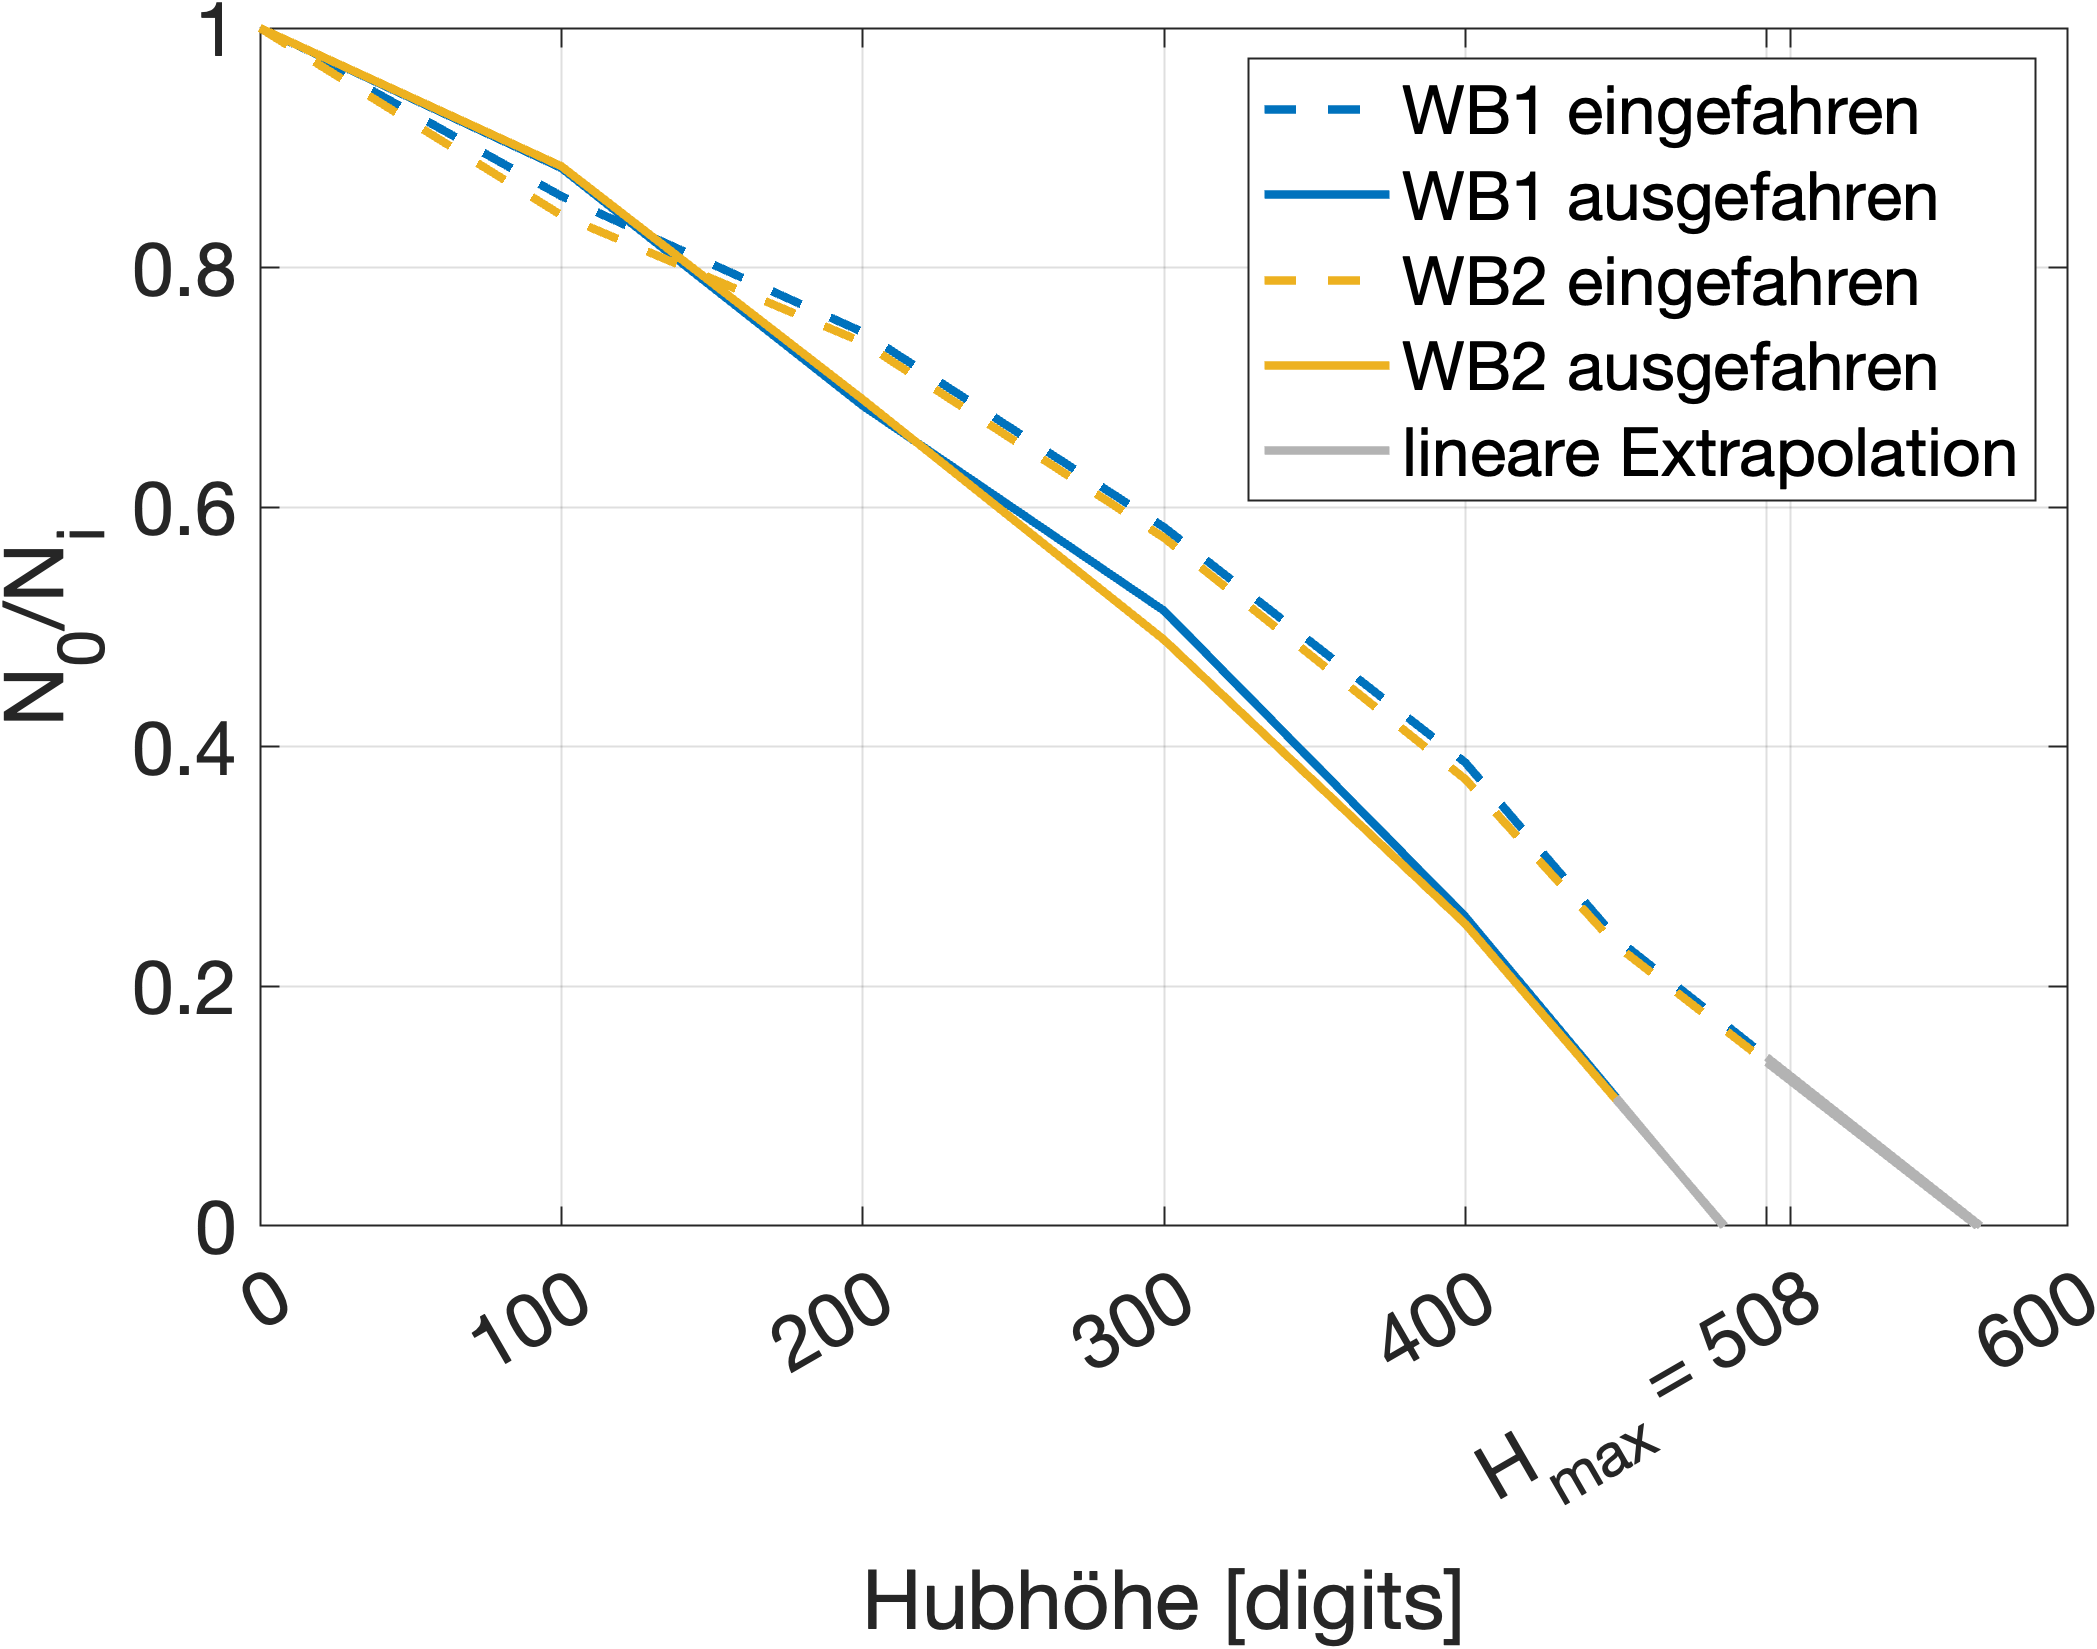
\includegraphics[width=0.7\textwidth]{relativeCount.png}
        \caption{Verlauf von $N_0 / N_i$}
        \label{fig:relativeCount}
    \end{figure}
    Wie in Abbildung \ref{fig:relativeCount} zu sehen ist, lässt sich aus den letzten zwei Messpunkten die ungefähren kritischen Positionen der unteren Kernhälfte extrapolieren.
    Bei eingefahrenen Steuerstäben ergibt sich eine kritische Hubhöhe von 571,5 digit (WB1) und 569,4 digit (WB2), bei ausgefahrenen Steuerstäben liegen die kritischen Positionen bei 485,4 digit (WB1) und 486,2 digit (WB2).

    \section{Auswertung}

    % Multiplikationsfaktor

    Aus der Veränderung der Neutronendichte lässt sich, mithilfe des initialen Werts, der Multiplikationsfaktor zu jeder Position der unteren Kernhälfte bestimmen. \\
    Aus den Messwerten lässt sich, wie in Tabellen 2 \& 3 eingetragen, der Multiplikationsfaktor berechnen:
    \begin{align*}
        k_0 &= 0.945 \\
        k_i &= 1 + \frac{N_{i-1}}{N_i} \cdot \left(k_{i-1} - 1\right)
    \end{align*}
    
    \begin{figure}[H]
        \centering
        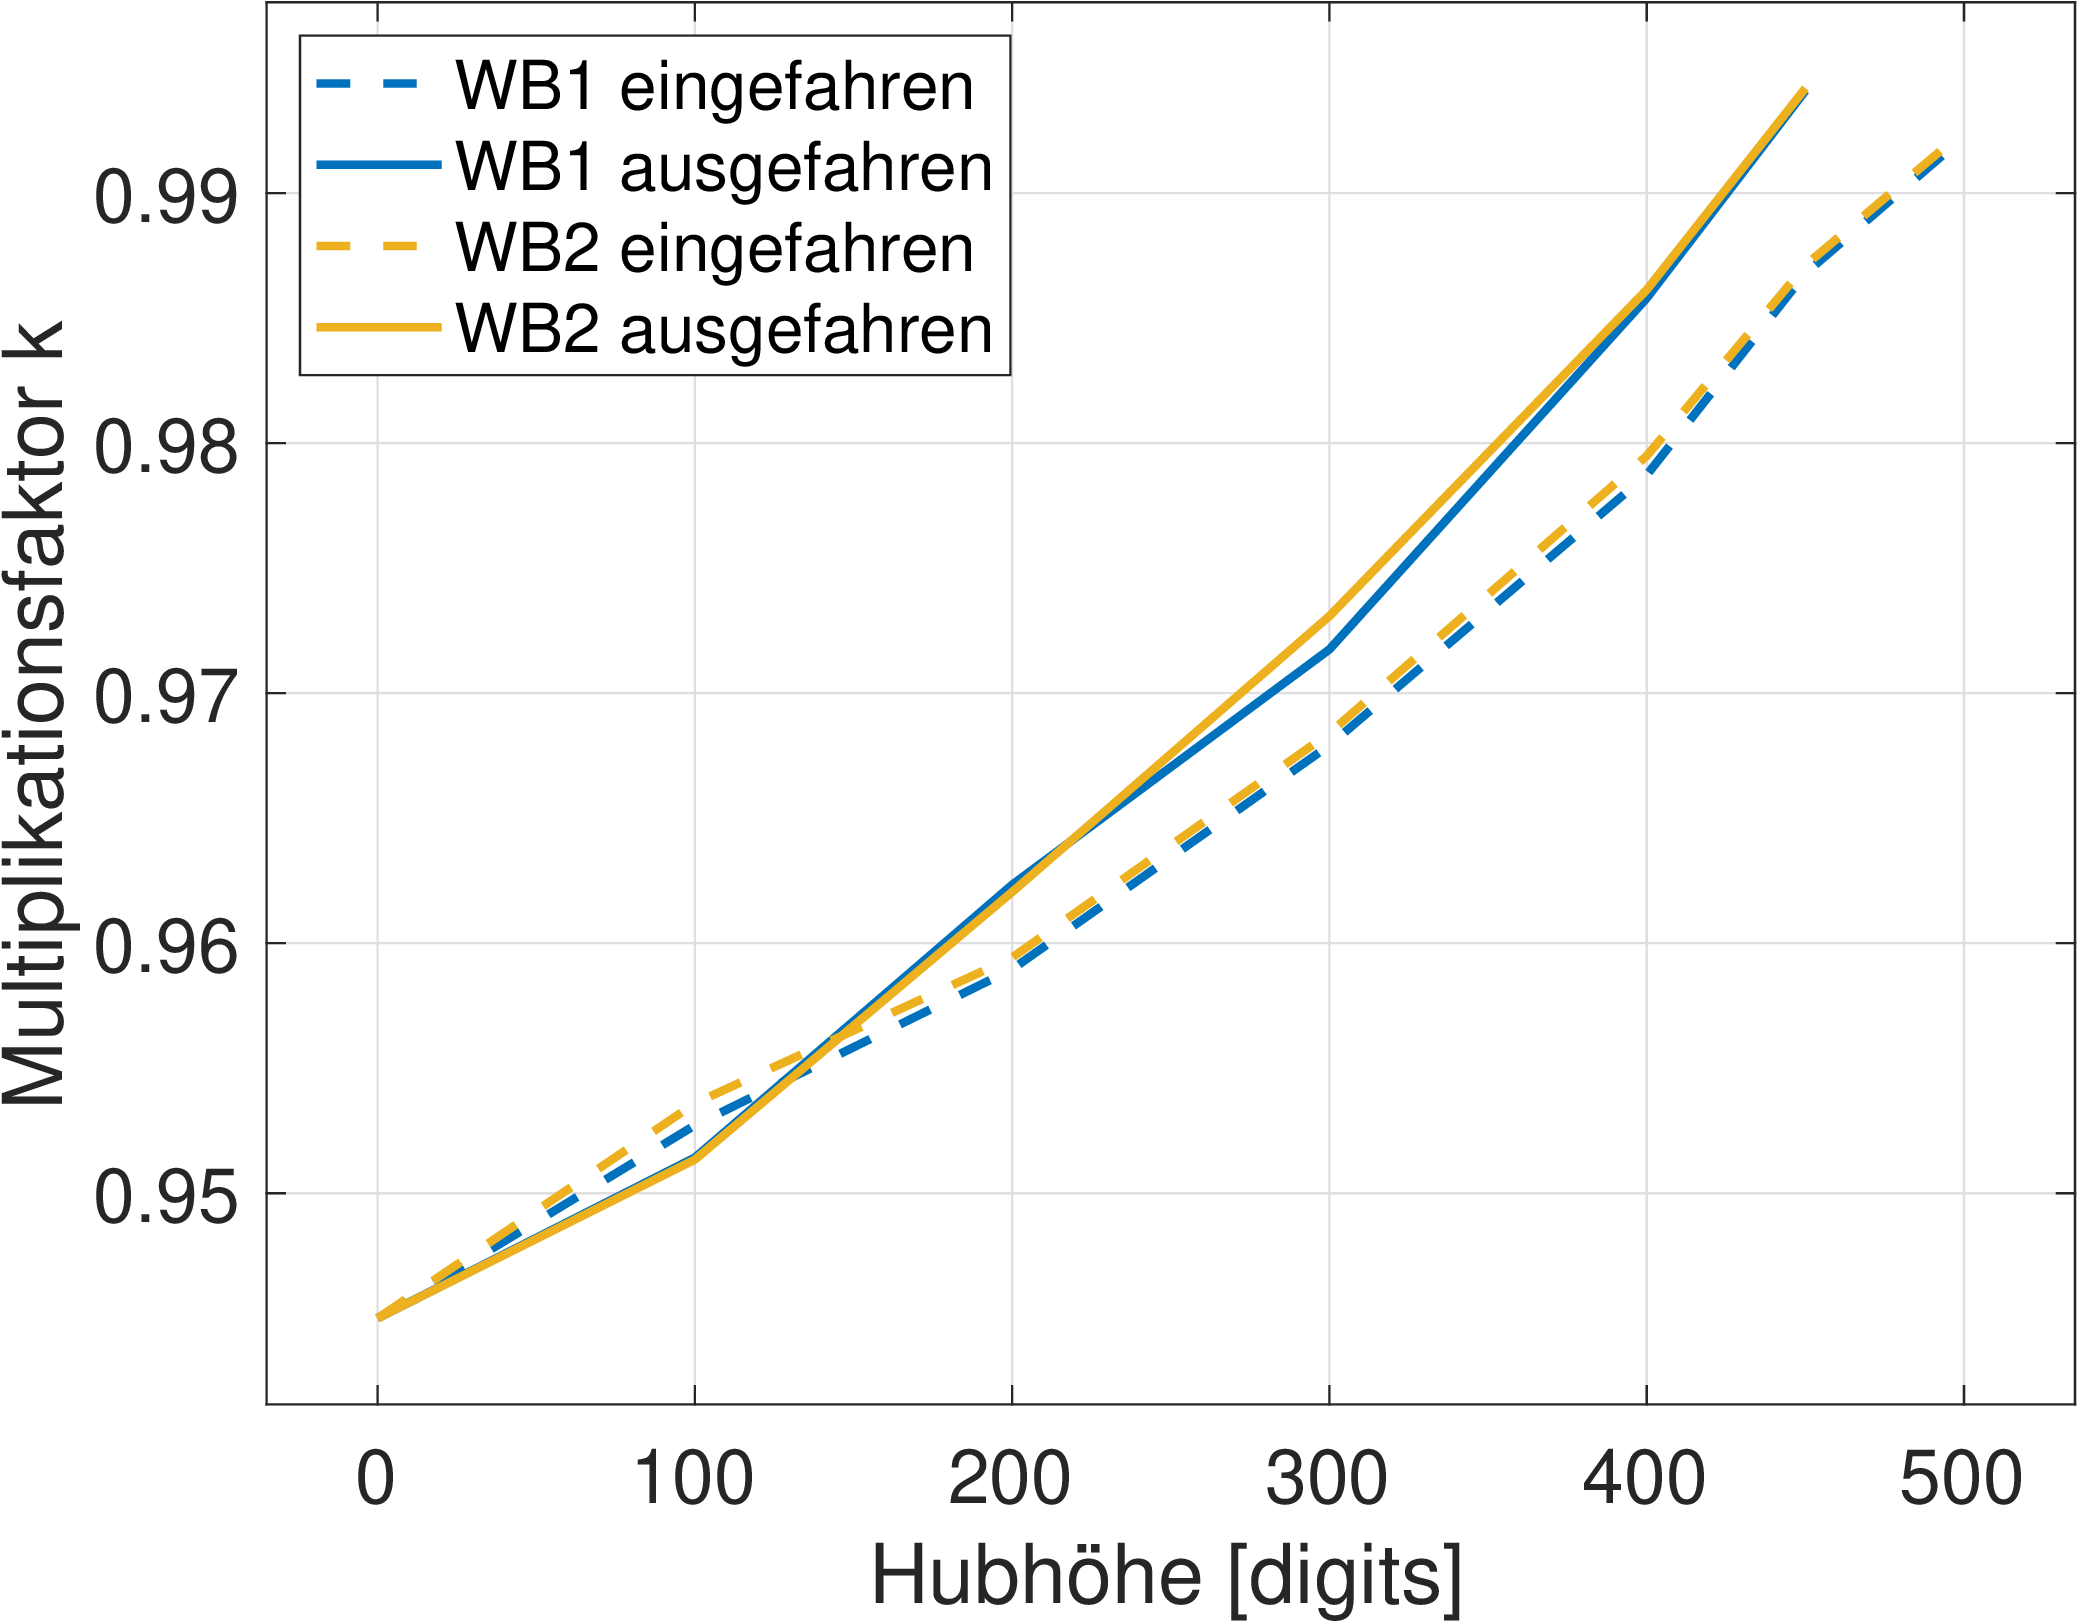
\includegraphics[width=0.7\textwidth]{multiplikationsfaktor.png}
        \caption{Multiplikationsfaktor}
        \label{fig:multFaktor}
    \end{figure}
    Wie in Abbildung \ref{fig:multFaktor} zu sehen ist, wächst der Multiplikationsfaktor stetig an, wobei er jedoch 1 nicht erreicht, da der Reaktor keinen kritischen Zustand erlangt.
    \\ \\
    % Unterkritische Verstärkung
    Aus dem Multiplikationsfaktor lässt sich ebenfalls berechnen, wie stark die unterkritische Verstärkung $M_i$ ist, die der Reaktor aufweist, wenn die Anfahrneutronenquelle eingefahren ist. \\
    Dabei bezeichnet die unterkritische Verstärkung den Parameter, der bestimmt, wie groß die asymptotische Neutronendichte nach unendlich langer Zeit ist, sofern die Quellstärke der Neutronenquelle und die Neutronengenerationszeit konstant sind.
    \begin{align*}
        M_i = \frac{1}{1 - k_i}
    \end{align*}

    \begin{figure}[H]
        \centering
        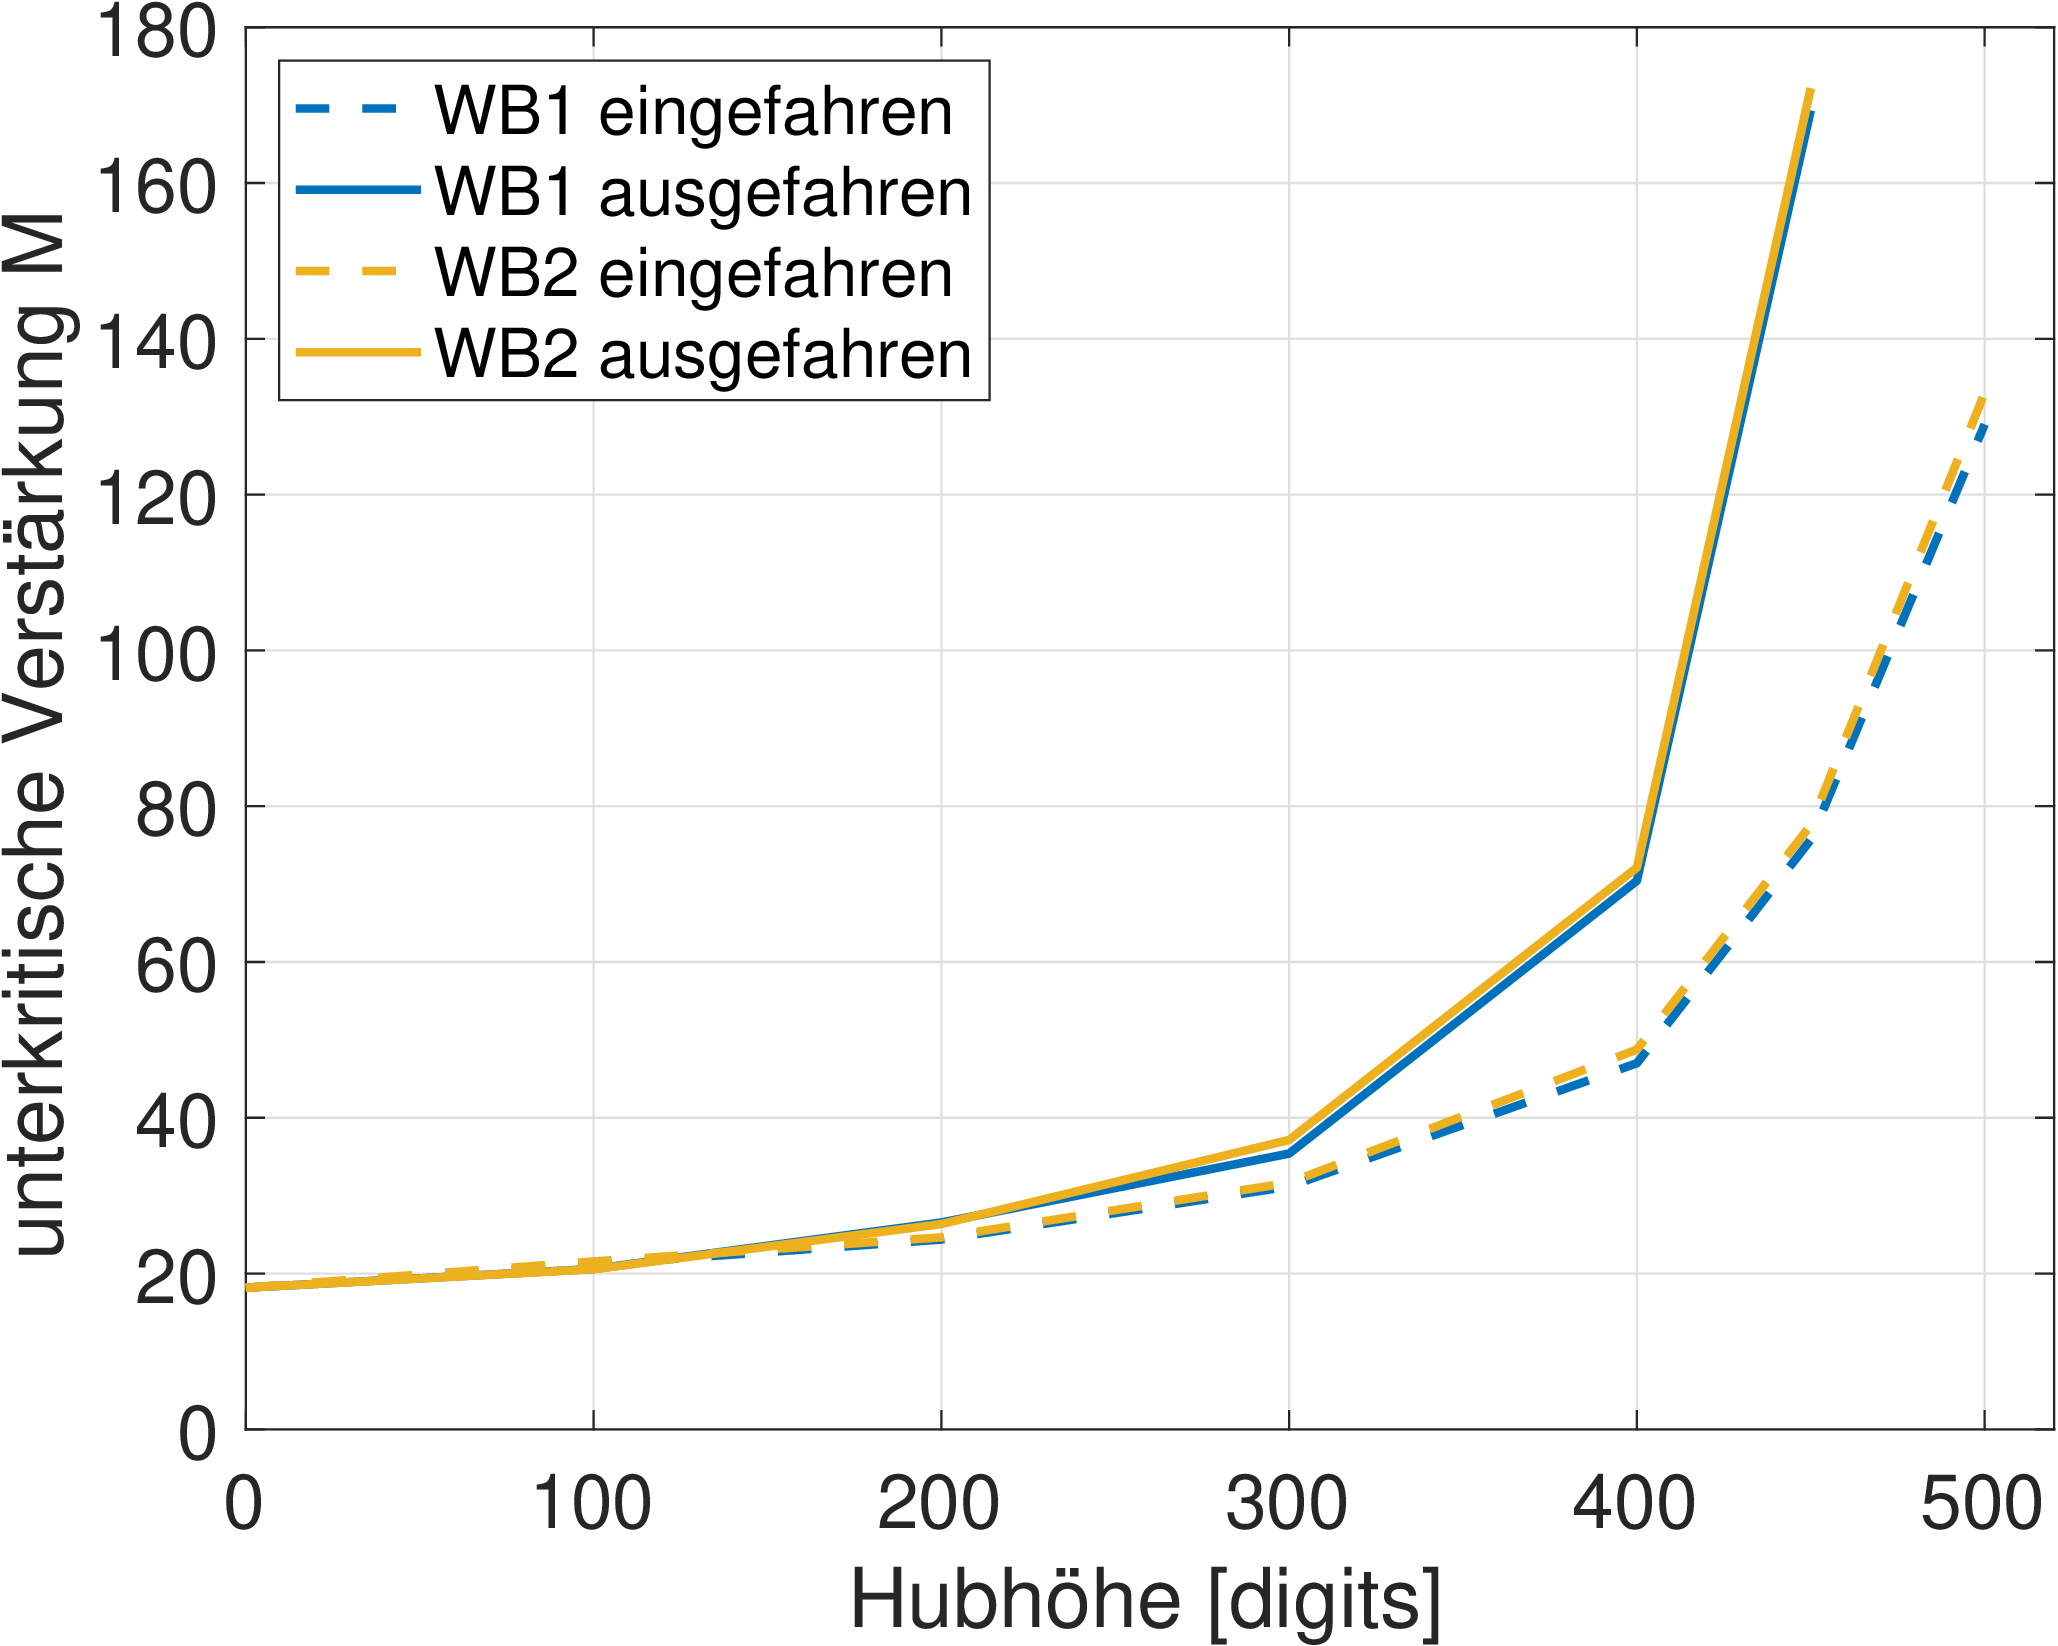
\includegraphics[width=0.7\textwidth]{unterkritischeVerstaerkung.png}
        \caption{unterkritische Verstärkung}
        \label{fig:unterkritVerst}
    \end{figure}
    Wie in Abbildung \ref{fig:unterkritVerst} zu sehen ist, wächst die unterkritische Verstärkung ins unendliche, wenn $k_i$ gegen 1 geht.
    \newpage
    % Reaktivität
    Weiterhin lässt sich aus dem Multiplikationsfaktor die Reaktivität berechnen:
    \begin{align*}
        \rho_i = \frac{k_i - 1}{k_i}
    \end{align*}

    \begin{figure}[H]
        \centering
        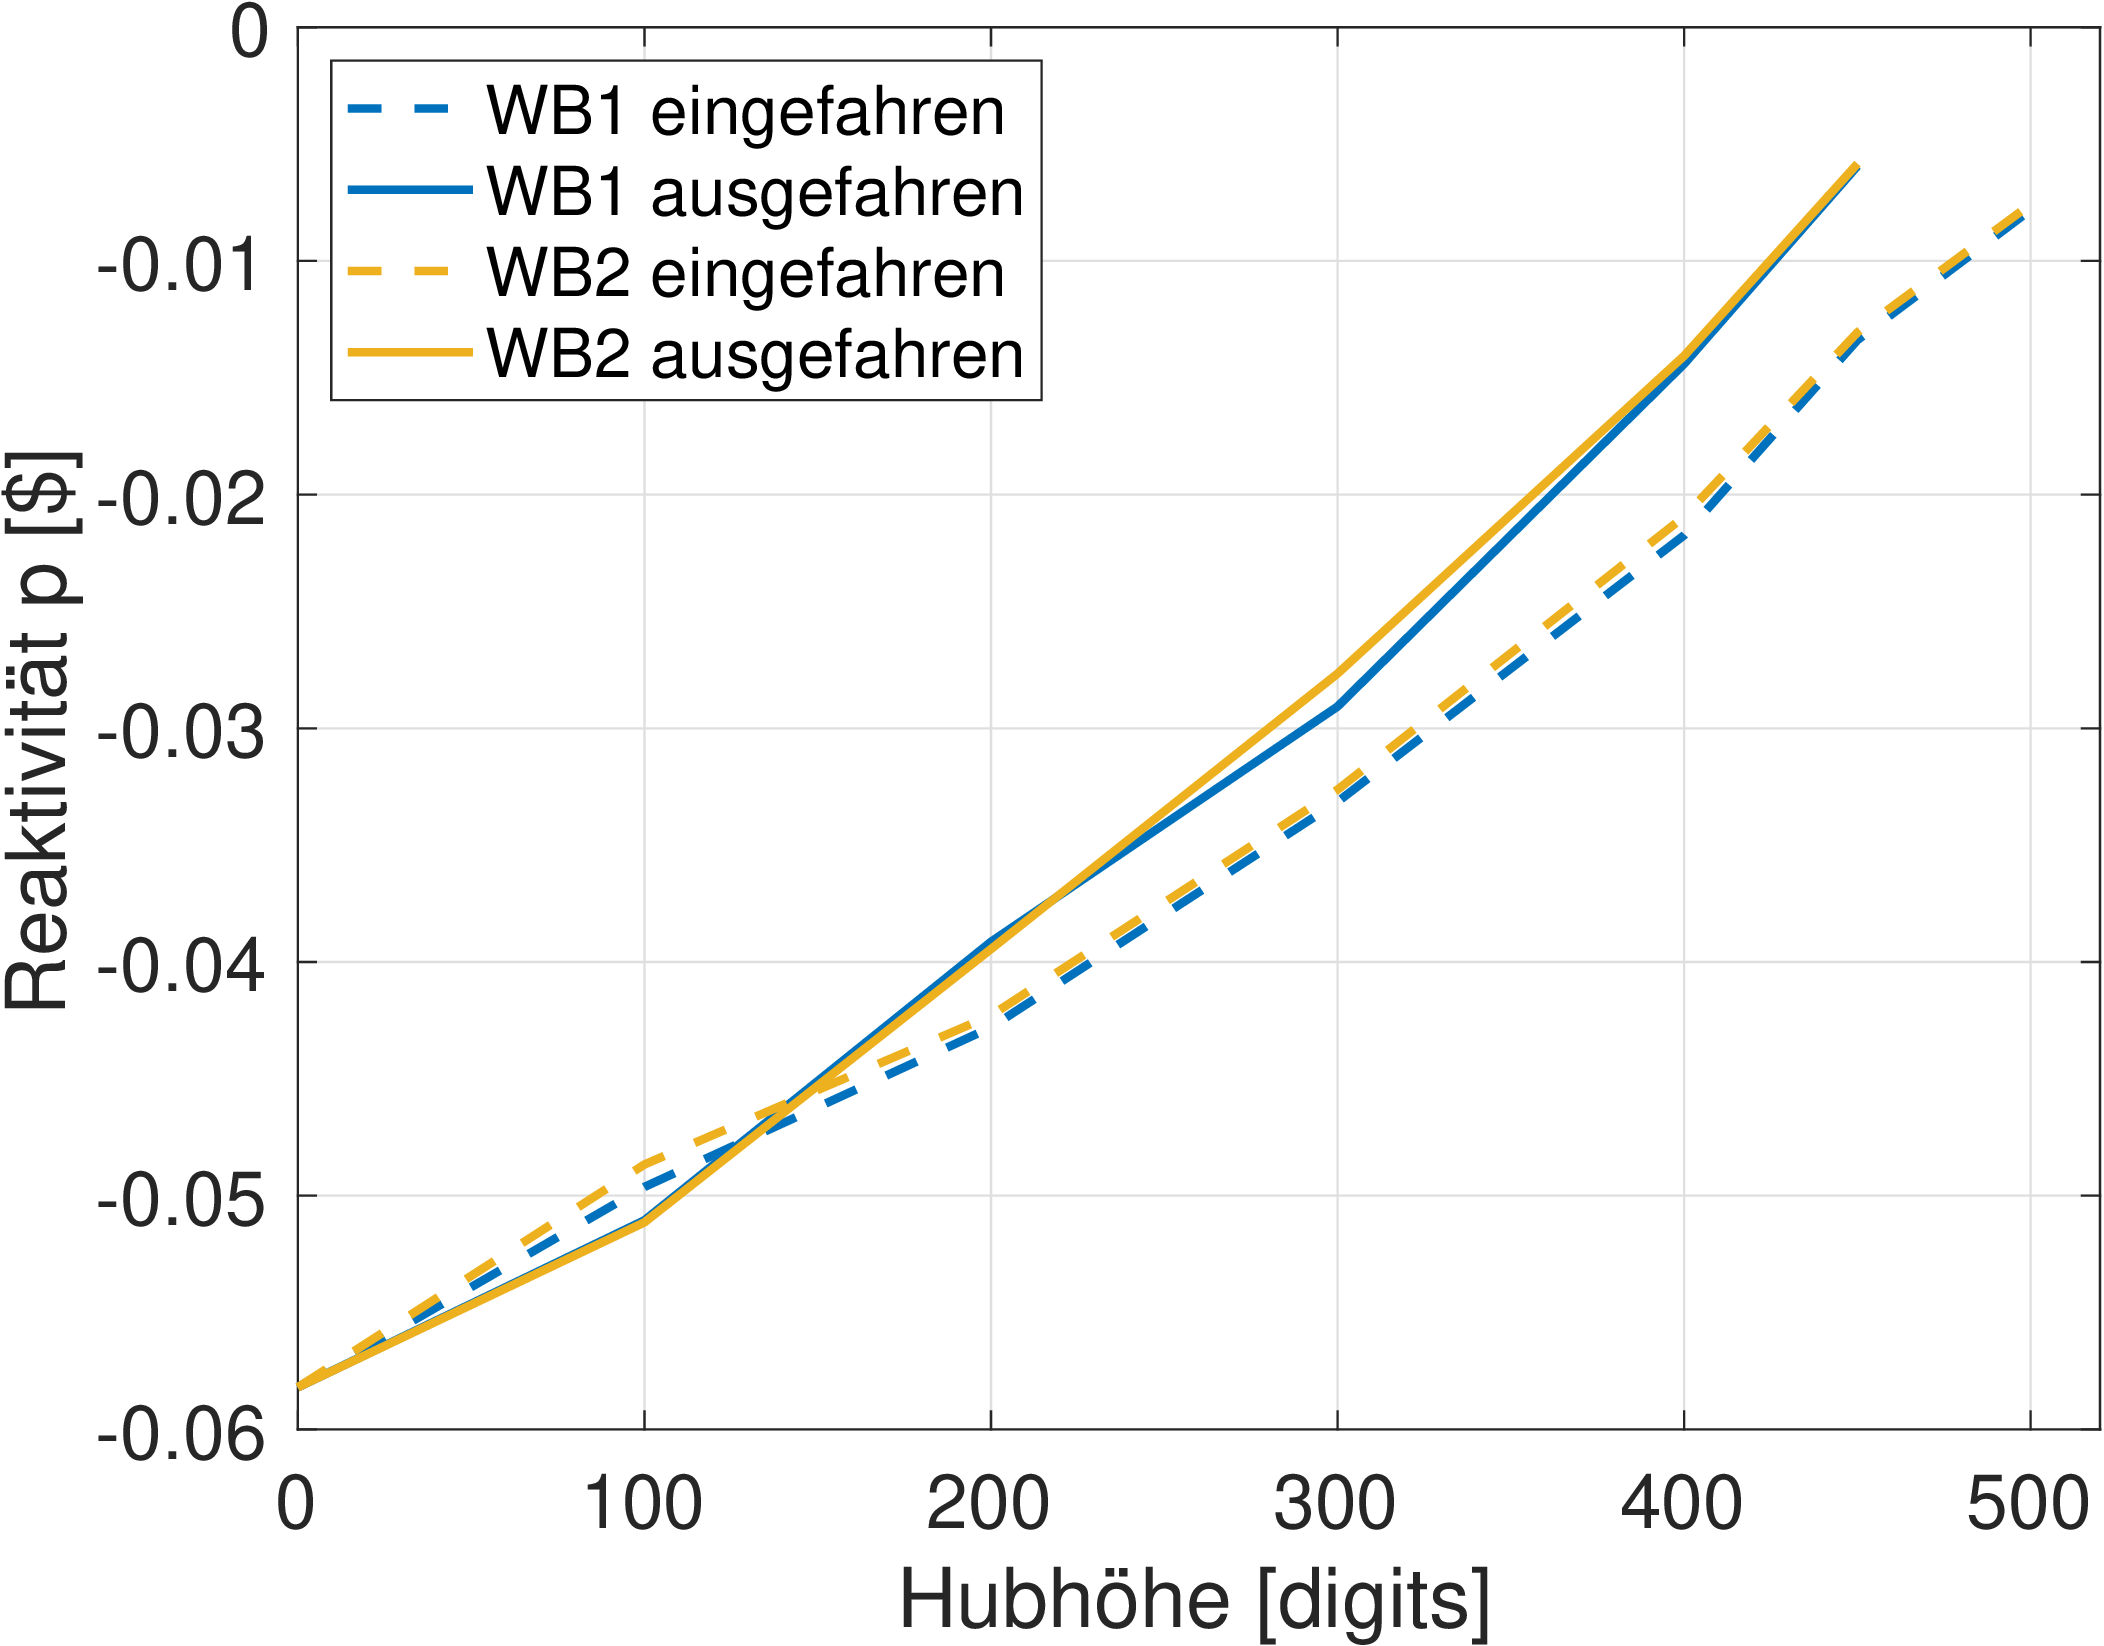
\includegraphics[width=0.7\textwidth]{reaktivitaet.png}
        \caption{Reaktivität}
        \label{fig:reaktivitaet}
    \end{figure}
    Wie in Abbildung \ref{fig:reaktivitaet} zu sehen ist nähert sich die Reaktivität an 0 an, was einem kritischen Zustand entspricht.

    \section{Fehlerbetrachtung}

    % Poisson-Verteilung Fehlergedöns
    \subsection{Statistischer Fehler}
    Die Neutronendetektoren unterliegen einem statistischen Fehler, da die Impulsrate der Neutronen ein statistischer Wert ist.
    Dabei berechnet sich der Fehler aus der Wurzel des Messwerts. \\
    Zu Beginn des Experiments liegen die Zählraten im Bereich von 8 - 12 Impulsen pro Sekunde. Damit liegt der Fehler bei $\pm\, 35\, \%$ bzw. $\pm\, 29\, \%$, was auch die Überkreuzung der Graphen in Abbildung \ref{fig:relativeCount} erklärt, welche in der Theorie nicht vorkommen sollte. \\
    Da die Zählraten am Ende des Experiments im Bereich von 95 Impulsen pro Sekunde liegen, womit der Fehler auf $\pm\, 10\, \%$ zurückgeht, hat sich die Sicherheit der Extrapolation entsprechend erhöht. \\
    Aus diesem Grund wird das Experiment in der Regel fortgeführt, bis die extrapolierten kritischen Parameterwerte mit Sicherheit die Ungleichung erfüllen.
    
    % Neutronendichte asymptotisch etc
    \subsection{Erreichen der asymptotischen Neutronendichte}
    Die Zeitabhängigkeit zum Erreichen der asymptotischen Neutronendichte n lautet
    \begin{align*}
        n(t) = \frac{S \cdot l}{1 - k} \cdot \left(1 - \exp \left[- \frac{1 - k}{l} \cdot t\right] \right)
    \end{align*}
    Aus der Gleichung ist ersichtlich, dass die Erreichung des asymptotischen Zustandes länger dauert, je näher sich der Reaktor an den kritischen Zustand annähert, der Multiplikationsfaktor also gegen 1 geht. \\
    Da bei Ausführen des Experiments jedoch nur begrenzt lange gewartet werden kann, wird die asymptotische Neutronendichte nie ganz erreicht, was zu einem weiteren Fehler führt.

    \newpage
    \section{Anhang}
    \begin{figure}[H]
        \centering
        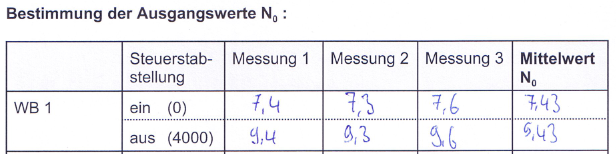
\includegraphics[width=0.7\textwidth]{ausgang_wb1.png}
        \caption{Ausgangswerte Weitbereichskanal 1}
    \end{figure}
    \begin{figure}[H]
        \centering
        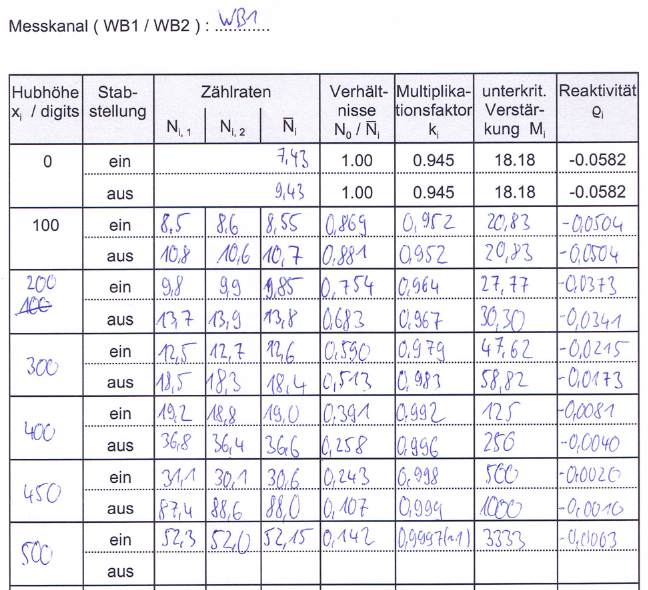
\includegraphics[width=0.9\textwidth]{messtabelle_wb1.png}
        \caption{Messtabelle Weitbereichskanal 1}
    \end{figure}
    \begin{figure}[H]
        \centering
        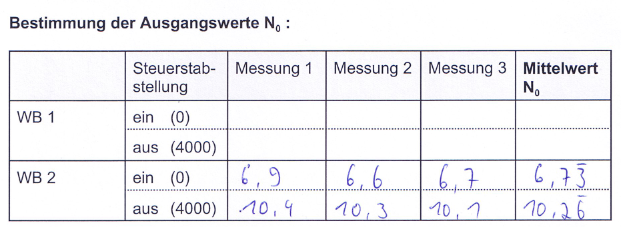
\includegraphics[width=0.7\textwidth]{ausgang_wb2.png}
        \caption{Ausgangswerte Weitbereichskanal 2}
    \end{figure}

    \begin{figure}[H]
        \centering
        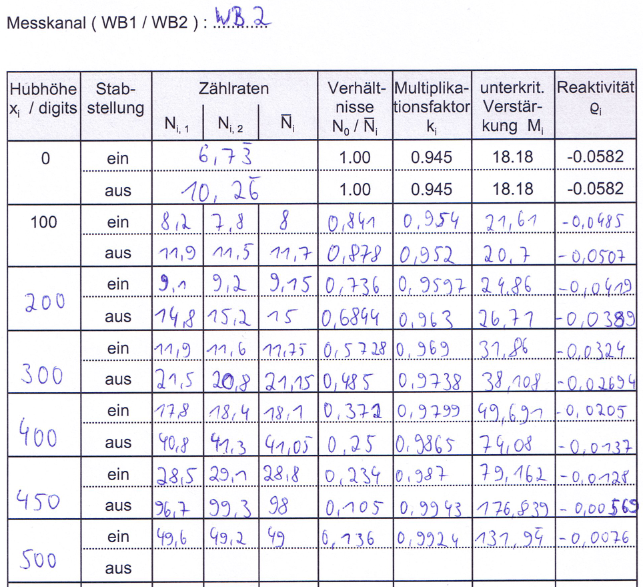
\includegraphics[width=0.9\textwidth]{messtabelle_wb2.png}
        \caption{Messtabelle Weitbereichskanal 2}
    \end{figure}
\end{document}